\documentclass[11pt]{article}
\usepackage[left=2cm, top=1.5cm, right=2cm, bottom=1.5cm]{geometry}
\usepackage[utf8]{inputenc}
\usepackage[T1]{fontenc}
\usepackage[french]{babel}
\usepackage{graphicx}
\usepackage{graphics}
\usepackage{amsmath}
\usepackage{tikz}
\usepackage{xcolor} 
\usepackage{mathtools}
\usepackage{parskip}
\usepackage{subcaption}
\usepackage[export]{adjustbox}
\usepackage{multicol}

\title{\vspace{-2cm}\textbf{TP 5 - Induction électromagnétique}}
\author{\vspace{-0.5cm}MENARD Alexandre - VIEILLEDENT Florent}
% \setlength{\parindent}{1cm}
\date{\vspace{-0.7cm}}


\newcommand{\ut}{\vec{u_\theta}}
\newcommand{\ur}{\vec{u_r}}
\newcommand{\uz}{\vec{u_z}}

\begin{document}
\maketitle

En présence d'un champ magnétique variable, un circuit électrique voit apparaître une tension à ses bornes, on parle d'induction électromagnétique.
Ce phénomène est aujourd'hui utilisé dans la charge par induction des smartphones, mais aussi dans les alternateurs et transformateurs électriques.
Dans ce travail pratique, nous proposons une étude qualitative et quantitative de la loi de Lenz-Faraday afin de vérifier sa cohérence avec l'expérience. 
Enfin, nous étudierons des transformateurs de tension, important pour optimiser le transport d'énergie électrique dans les réseaux.

\section{Loi de Lenz-Faraday en champ variable}
\subsection{Théorie}
Dans le cadre de ce travail pratique, nous nous placerons dans l'approximation des régimes quasi-stationnaires, le courant
sera donc le même partout dans un même circuit, et l'on négligera les temps de propagation du champ magnétique entre les deux circuits.
Soit 2 bobines de diamètre $d$ et de nombre de spires $N_H$ placées à une distance $d/2$ l'une de l'autre, et parcourues par un courant $i(t) = i_0\sin(\omega t + \psi)$.	
On a alors le flux magnétique au travers d'une bobine à section carré de côté $a \in [a_{min}, a_{max}]$ :
\begin{align}
    \label{eqn:relation_1}
    \Phi(t) & = \overbrace{\left(\frac{4}{5} \right)^{\frac{3}{2}} \frac{2\mu_0 N_H}{d}}^{\alpha} \overbrace{\left(\frac{a_{min}^2 + a_{max}^2 + a_{min}a_{max}}{3}\right)}^{S} N \cos \theta i(t) \nonumber\\
    & = \alpha S N i(t)
\end{align}
On en déduit alors la force électromotrice induite (f.e.m) dans la bobine carrée:
\begin{align}
    e(t) = -\frac{d\Phi(t)}{dt} = -\alpha S N \omega \cos \theta i_0 \cos (\omega t + \psi) = \alpha S N \omega \cos \theta i_0 \sin (\omega t + \psi - \frac{\pi}{2})
\end{align}

On s'attend alors à ce que le déphasage entre $e(t)$ et $i(t)$ soit de $\frac{\pi}{2}$, avec $e(t)$ qui sera en retard. Enfin, $e(t)$ est proportionnel
à $N$, $\omega$ et $\cos \theta$.

Enfin, pour déterminer l'inductance mutuelle $M$, on a:
\begin{align}
  \label{eqn:relation_M}
  \frac{e}{i} = \alpha S N \omega \text{ et } M = \frac{\Phi_{1 \rightarrow 2}}{ i} = \alpha S N \Rightarrow \frac{e}{i} = M \omega
\end{align}

\subsection{Montage expérimental et détermination des incertitudes}
On installe 2 bobines de Helmholtz de diamètre $d = 13cm$, avec $N_H = 95 spires$, que l'on sépare d'une distance $d/2$. On les installe en série sur la sortie
à $50\Omega$ d'un GBF, puis en sortie de la dernière, on relie à l'oscilloscope, puis l'on termine le circuit sur la masse de la sortie du GBF. 
On installe ensuite au centre des deux bobines, une troisième bobine dite inductive de section $S$ (voire (\ref{eqn:relation_1})) dont on relie les bornes à l'oscilloscope.

Pour relever les tensions $U_1$ (bobines de Helmholtz) et $U_2$ (bobine inductive), on utilise l'onglet "Mesure" de l'oscilloscope, et l'on récupère la valeur maximale
de $U_1$ et $U_2$. On utilisera une incertitude de $3\%$ pour les mesures de tension (d'après le manuel), et pour le temps, nous utilisons les curseurs en faisant la moyenne des valeurs maximales
et minimales. Pour obtenir le déphasage, on relève l'écart de temps $\Delta t$ entre un pic de $U_1$ et $U_2$ (succesifs). On utilise ensuite la formule suivante pour calculer le déphasage avec $T = 1/\nu$ :

\begin{equation}
    \psi = \frac{\Delta t}{T} \times 2\pi
\end{equation}

\subsection{Déphasage et inductance mutuelle}
On applique alors un courant sinusoidal de fréquence $\nu \in [200\text{Hz}; 10\text{kHz}]$ avec une incertitude $\delta \nu = 1Hz$, et l'on relève $U_1, U_2, \Delta t$ pour une bobine de $N_1 = 1000$ spires ainsi qu'une bobine de $N_2 = 500$ spires. 
On trace alors le rapport $e/i$ en fonction de $\omega$:

\begin{figure}[h!]
    \centering
    \begin{subfigure}{.5\textwidth}
      \centering
        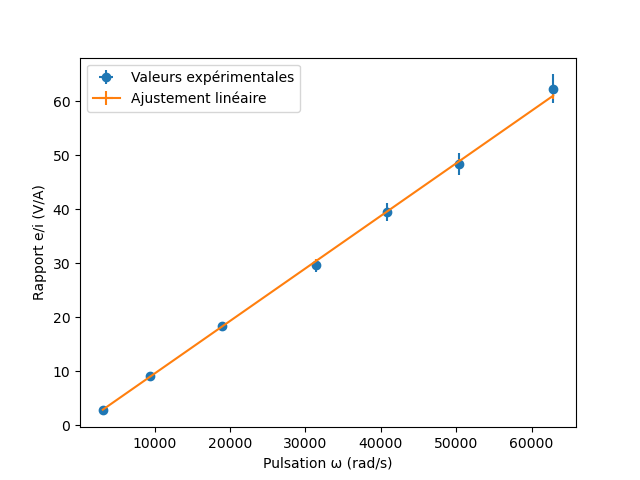
\includegraphics[width=.95\linewidth]{img/Graph_1000spires.png}
      \caption{Avec $1000$ spires}
      \label{fig:sfig1}
    \end{subfigure}%
    \begin{subfigure}{.5\textwidth}
      \centering
      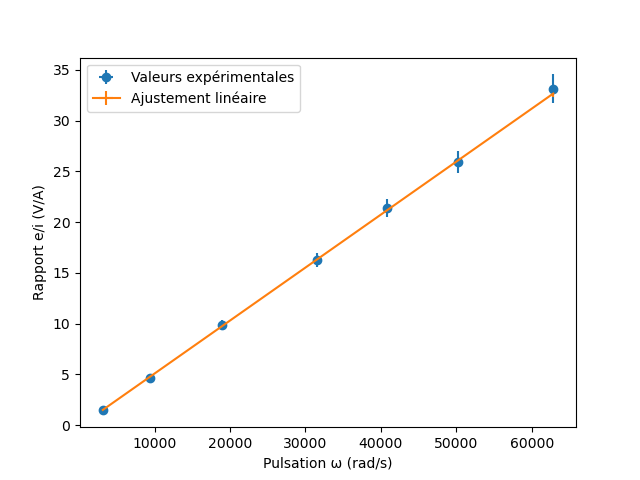
\includegraphics[width=.95\linewidth]{img/Graph_500spires.png}
      \caption{Avec $500$ spires}
      \label{fig:sfig2}
    \end{subfigure}
\end{figure}

Par régression linéaire nous obtenons $M$ d'après (\ref{eqn:relation_1}):
\begin{align}
    \text{1000 spires: } M_1 = (9.74 \pm 0.09) \times 10^{-4} V.A^{-1}.s^{-1}, b_1 = -0.16 \pm 0.07 V.A^{-1} \\
    \text{500 spires: } M_2 = (5.22 \pm 0.05) \times 10^{-4} V.A^{-1}.s^{-1}, b_2 = -0.14 \pm 0.04 V.A^{-1}
\end{align}

On remarque un premier écart à la théorie, on obtient une ordonnée à l'origine non nulle, ce qui n'est pas prédit car pour une fréquence nulle, le champ $\vec{B}$
ne varie plus, on ne devrait donc plus observer de f.e.m. Cependant, la présence de cette f.e.m résiduelle peut s'expliquer par la présence d'appareils et de câbles proches
générant un champ magnétique localement. On pourrait régler ce problème en installant le montage entre deux plus grandes bobines de Helmholtz de telle sorte
qu'elles compensent tous les champs magnétiques présents.

Concernant les valeurs d'inductance mutuelle $M_1, M_2$, on doit obtenir théoriquement:
\begin{align*}
  M_{th,1} = (1.06 \pm 0.05) \times 10^{-3} V.A^{-1}.s^{-1} \\
  M_{th,2} = (5.2 \pm 0.3) \times 10^{-4} V.A^{-1}.s^{-1}
\end{align*}

La valeur de $M_{th,2}$ se retrouve dans notre valeur $M_2$, cependant, $M_1$ et $M_{th,1}$ ne se retrouvent pas dans les incertitudes bien que les valeurs ne soient pas 
très éloignées. Il serait donc intéressant de répéter la mesure pour déterminer un écart-type de notre valeur de $M_1$ et vérifier si l'on retrouve $M_{th,1}$ dans l'intervalle de confiance.

Enfin, concernant le déphasage, pour le montage avec $1000$ spires, on observe un déphasage compris entre $89 \pm 0.9 ^{\circ}$ et $93.7 \pm 0.9 ^{\circ}$ et pour $500$ spires, on a 
un déphasage compris entre $90.7 \pm 1 ^\circ$ et $95.7 \pm 1 ^\circ$. On observe aucune corrélation entre déphasage et modification des paramètres, nous supposons donc 
que cet écart à la théorie est simplement dû une incertitude sur le temps potentiellement sous-estimée, il serait préférable de réaliser un calcul de déphasage numériquement en récupérant
la liste de valeurs de $U_1$ et $U_2$ pour obtenir un décalage temporel plus précis.


\break
\subsection{Influence de l'orientation}
On reprend le montage expérimental, mais on oriente la bobine inductive de $1000$ spires de telle sorte à ce qu'elle face un angle $\theta$ avec l'axe des 2 bobines.
On repère l'angle à partir d'un cercle gradué, on estime ainsi l'incertitude à $\delta \theta = 5^{\circ}$. On positionne le GBF à $\nu = 3003.6 \pm 5 Hz$ et l'on relève la f.e.m
comme dans la partie précédente. On trace alors la f.e.m en fonction de $\cos \theta$:

\begin{figure}[h!]
  \centering
  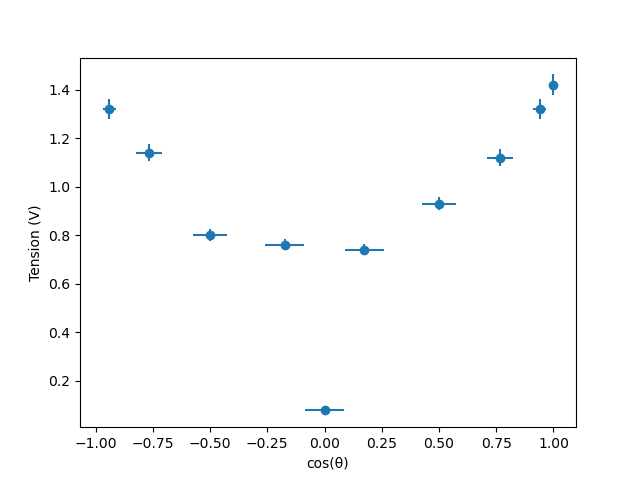
\includegraphics[width=.5\linewidth]{img/Graph_Angle.png}
  \caption{Avec $500$ spires}
  \label{fig:graphe_angle}
\end{figure}

On remarque que les pour des angles extrémaux loin de $90^{\circ}$, on obtient bien un comportement linéaire de la tension en fonction de $\cos \theta$,
cependant, plus on s'approche de l'angle $\theta = 90^{\circ}$, on observe une déviation à la théorie. Cet écart s'explique par $e(t)$ qui présente une forte
sensibilité à l'angle $\theta$ à l'approche de $90^{\circ}$, une légère variation pouvant faire doubler la mesure. Il est donc clair que notre incertitude sur la tension est sous-estimée
car ne prend pas en compte cet aspect de la mesure. De plus, le flux est dépendant du centragre de la bobine inductive, ainsi que de l'angle qui n'est pas précis dans le montage.
Il faudrait utiliser un montage capable d'orienter précisèment la bobine inductive, et de façon fixe car un expérimentateur devait maintenir manuellement la bobine, sinon les fils 
repousser la bobine. 

Ainsi, nous pouvons simplement affirmer que l'on observe une tension presque nulle pour un angle $\theta = 90^{\circ}$, et que la théorie prédit correctement l'aspect qualitatif de la f.e.m pour des angles faibles.
L'absence de symétrie de nos mesures ne nous permet pas de les prendre en compte pour une analyse plus en détails car l'ensemble de nos tensions pourraient être mauvaises.

\subsection{Cas d'un courant "triangulaire"}
On reprend le montage expérimental initial avec une bobine inductive à $1000$ spires, au centre des deux bobines. On passe le GBF en signal triangulaire et l'on fixe la fréquence
à $\nu = 200 \pm 1 Hz$. On observe (voir figure \ref{fig:oscillo}) bien un signal triangulaire pour $U_1$, mais la bobine inductive subit une f.e.m suivant un signal carré, et l'on remarque
que sur les ascendants du signal triangulaire, la f.e.m est négative et constante; et sur les descendants du signal triangulaire, la f.e.m est positive et constante.
Cette observation est cohérente car sur un ascendant de $U_1$, on a une pente constante positive, d'où une f.e.m négative constante ($-\frac{d\Phi}{dt}$), et inversement sur un descendant.
Fait notable, nous ne notons pas de déphasage entre les deux signaux par rapport à un signal sinusoïdal.

\break
\section{Transformateurs de tension}
PSAHTEK JE REDIGE MERCREDI SOIR


\break
\section*{Annexes}
\subsection{Cas d'un courant "triangulaire"}
\begin{figure}[h!]
  \centering
  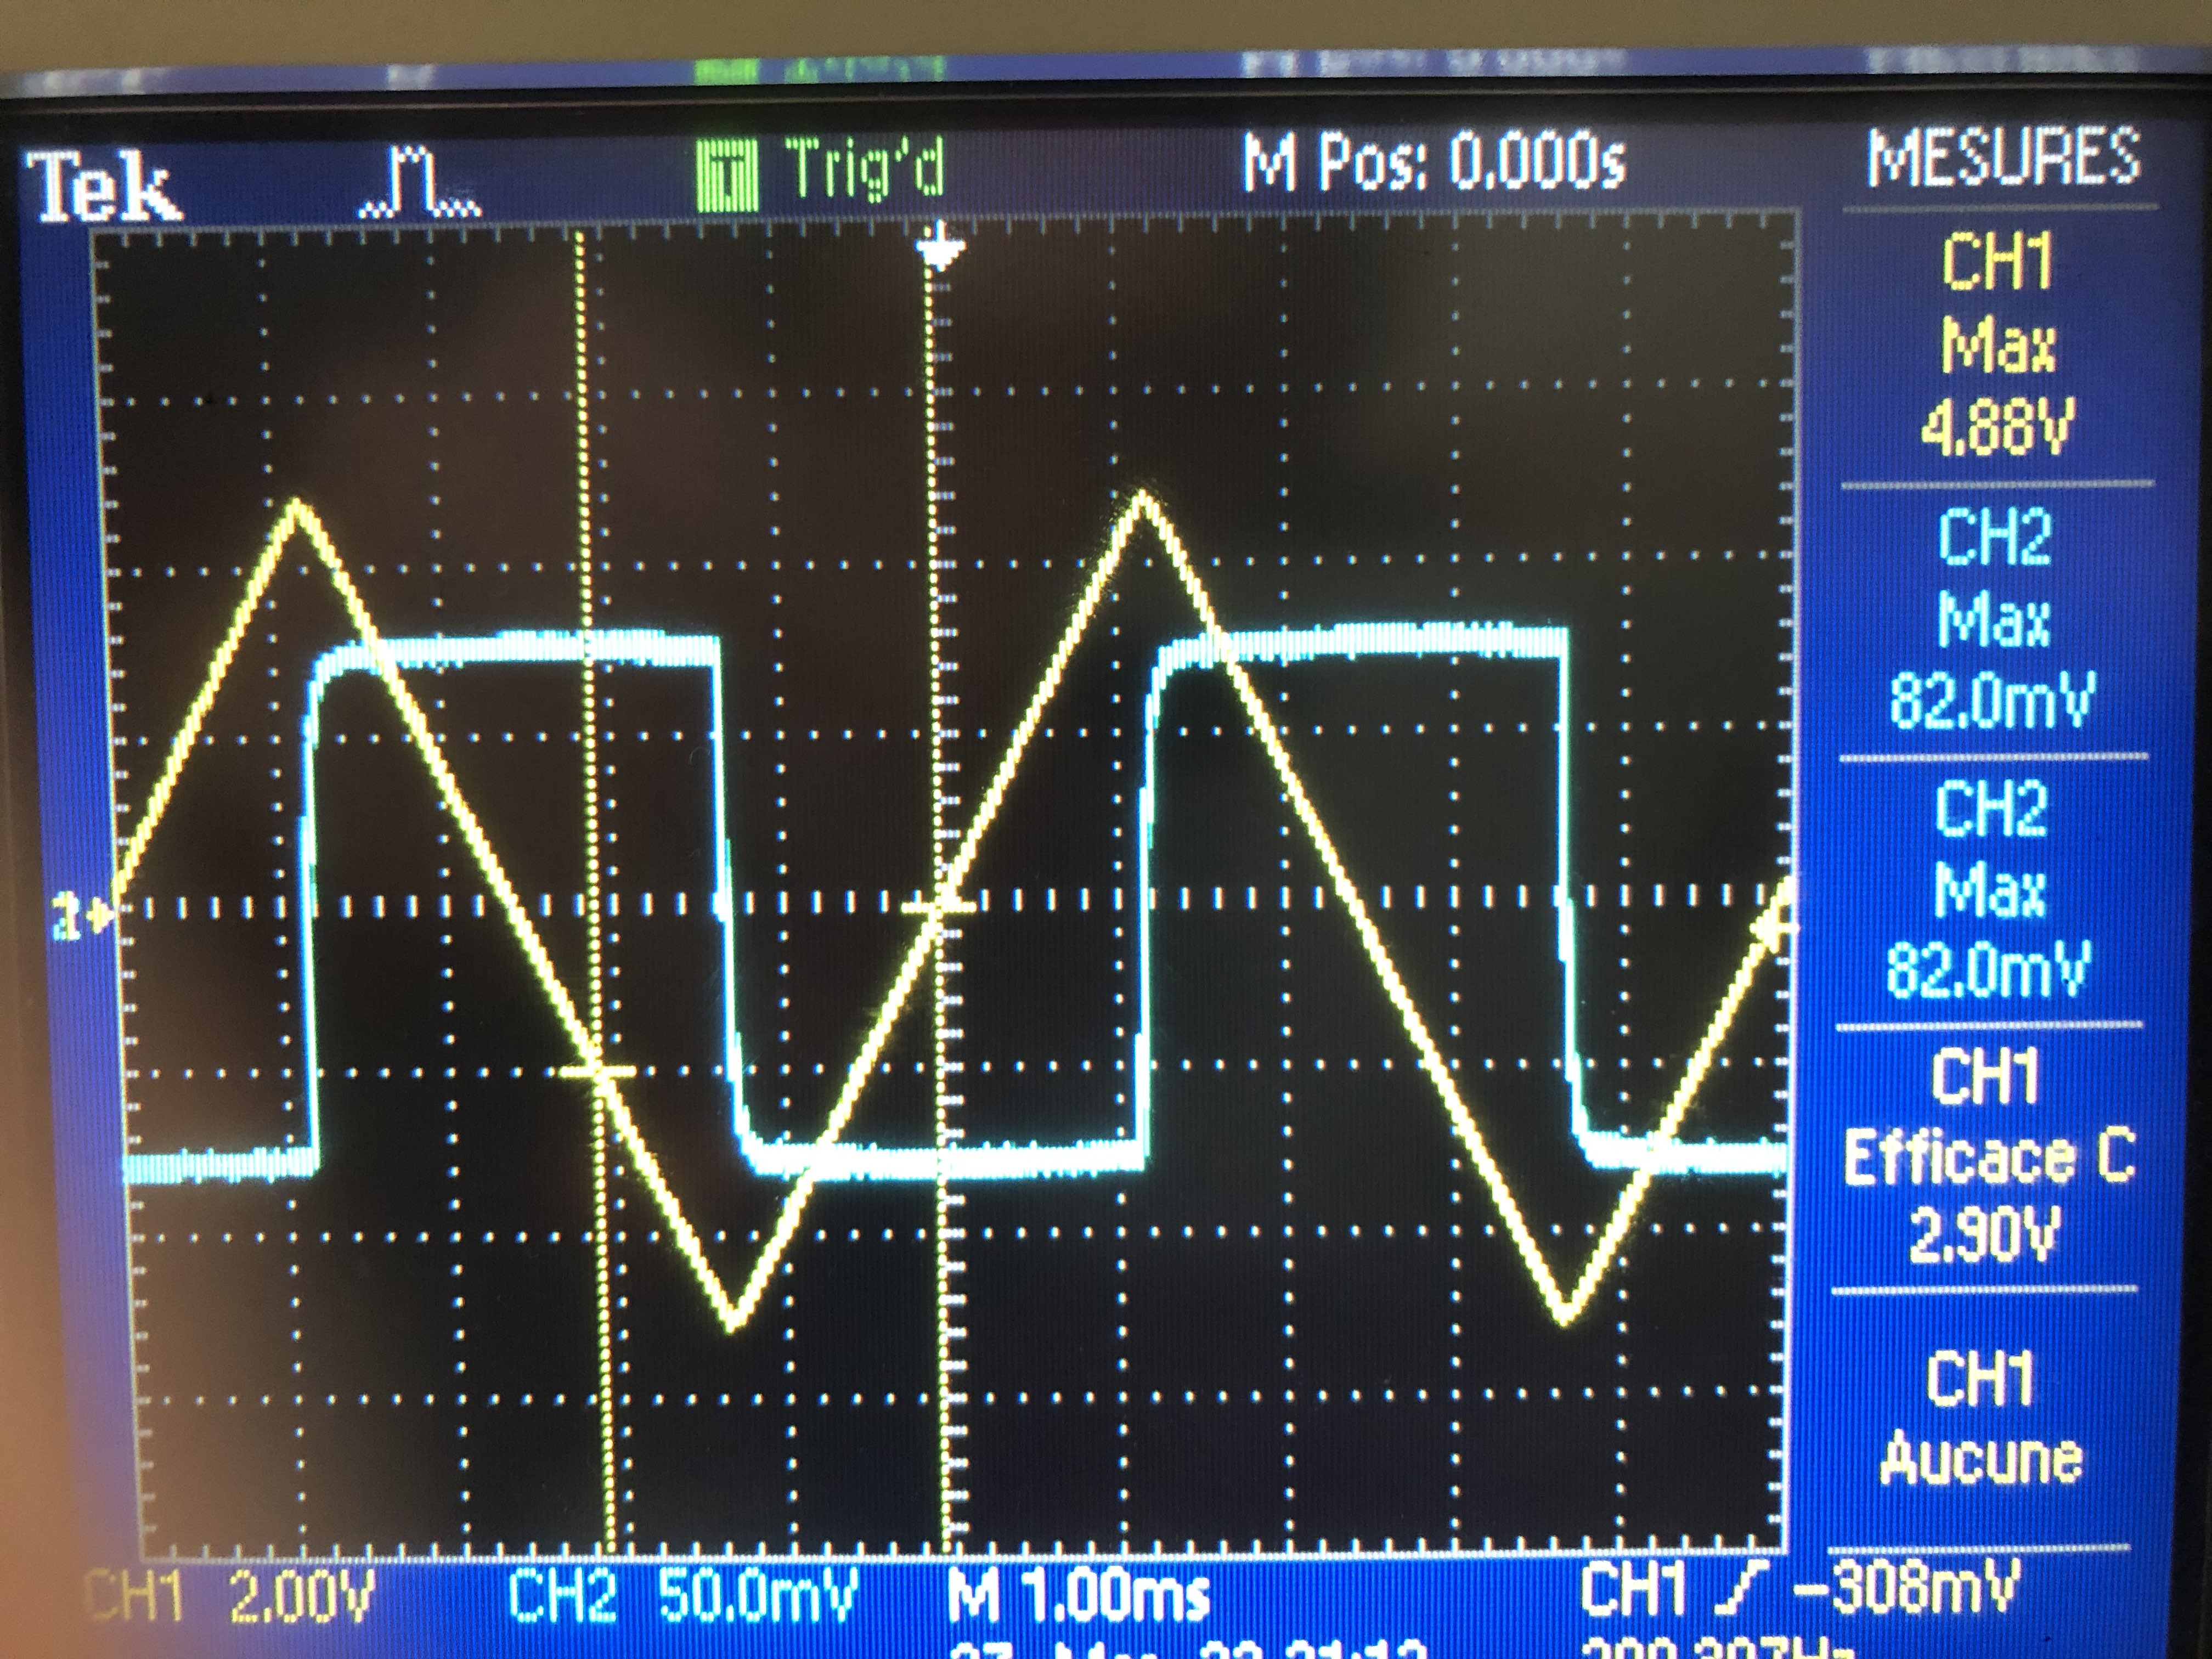
\includegraphics[width=.5\linewidth]{img/oscillo.png}
  \caption{Tension mesurée pour les deux circuits}
  \label{fig:oscillo}
\end{figure}

Le signal jaune représente $U_1$, la tension du circuit contenant la bobine de Helmholtz, et le signal bleu représente la f.e.m.


\end{document}